\documentclass[12pt, a4paper]{article}  

\usepackage{etex} % расширение классического tex в частности позволяет подгружать гораздо больше пакетов, чем мы и займёмся далее

%%%%%%%%%% Математика %%%%%%%%%%
\usepackage{amsmath,amsfonts,amssymb,amsthm,mathtools} 


%%%%%%%%%%%%%%%%%%%%%%%% Шрифты %%%%%%%%%%%%%%%%%%%%%%%%%%%%%%%%%
\usepackage{fontspec}         % пакет для подгрузки шрифтов
\setmainfont{Arial}   % задаёт основной шрифт документа

\defaultfontfeatures{Mapping=tex-text}

\newfontfamily{\cyrillicfonttt}{Arial}
\newfontfamily{\cyrillicfont}{Arial}
\newfontfamily{\cyrillicfontsf}{Arial}

\usepackage{unicode-math}     % пакет для установки математического шрифта
\setmathfont{Phorssa}      % шрифт для математики

\usepackage{polyglossia}      % Пакет, который позволяет подгружать русские буквы
\setdefaultlanguage{russian}  % Основной язык документа
\setotherlanguage{english}    % Второстепенный язык документа


%%%%%%%%%% Работа с картинками %%%%%%%%%
\usepackage{graphicx}                  % Для вставки рисунков
\usepackage{graphics} 
\graphicspath{{pop-art/},{pictures/}}    % можно указать папки с картинками
\usepackage{wrapfig}                   % Обтекание рисунков и таблиц текстом
\usepackage{subfigure}                 % для создания нескольких рисунков внутри одного
\usepackage{rotating}


%%%%%%%%%% Работа с таблицами %%%%%%%%%%
\usepackage{tabularx}            % новые типы колонок
\usepackage{tabulary}            % и ещё новые типы колонок
\usepackage{array}               % Дополнительная работа с таблицами
\usepackage{longtable}           % Длинные таблицы
\usepackage{multirow}            % Слияние строк в таблице
\usepackage{float}               % возможность позиционировать объекты в нужном месте 
\usepackage{booktabs}            % таблицы как в книгах!  
\renewcommand{\arraystretch}{1.3} % больше расстояние между строками
\usepackage[landscape,top=2mm, bottom=2mm,left=2mm,right=2mm,includefoot]{geometry}

\DeclareMathOperator{\diag}{diag}  % математический оператор, который описывает диагональную матрицу


%заголовок

\author{Никаноров Иван}
\title{Домашняя работа №2. Задание 3}
\date {\today}

\begin{document}

\maketitle

\newpage

 \begin{center}
 \section{Угроза}
 \end{center}
\Large{\fontspec{Phorssa}{Ульянкин Филипп, позволь познакомить тебя с моим другом из сериала "Визитёры" (не знаю, смотрел ты его или нет... Впрочем, это не важно, я тебе напомню тогда об этом милом создании, если смотрел.)}}
 \begin{figure} [H]
  \begin{center}
  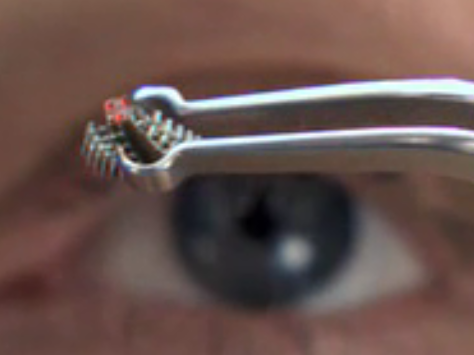
\includegraphics[scale=0.55]{Cleaner.png}
  \end{center}
 \end{figure}
\Large{\fontspec{Phorssa}{Зовут эту маленькую тварь "Чистильщик" (по крайней мере, согласно нашим переводчикам. Как в оригинале он называется, сказать не рисну). Чистильщик проникает внутрь человека через голову и начинает исследовать тело носителя, двигаясь, почему-то, вдоль нервов. Боль, которую он при этом вызывает, я думаю, похожа на ту, что испытывал бы, если бы к каждому участку нерва последовательно, шаг за шагом, прикладывали раскалённый кусочек железа. Исследовав всё, что можно исследовать, он выходит через мягкие ткани (обычно через репродуктивные органы)... 
В общем, носителю он доставляет такие мучения, что он начинает умолять о смерти! Филипп, если ты ещё раз в домашку подкинешь такую свинью, как второй номер, который сжирает кучу времени, то однажды ночью проснёшься от того, что мой маленький друг залезает тебе в глаз!}}

\newpage %не знаю почему, но без этой строчки он ругается, хотя pdf-ку спокойно делает
\begin{center}
\section{Формулы}
\end{center}

$$2+2=5$$
$$\sin(15x)$$
$$\sum_{i=1}^{n} x^i$$
$$\int_a^b f(x)dx$$
$$\epsilon$$
$$\lim_{n \to a} \frac{1}{n}$$

Набираться будут числовые формулы, формулы со знаком суммы, те, в которых используются математические операторы, набранные прямым шрифтом (не курсивом)и формулы с дробями. Соответственно, не будут набираться формулы, в которых используется курсив, стрелки или знак интеграла, дроби. Происходит это потому, что данный шрифт не поддерживает курсив, стрелку, знак интеграла и т.д. (хотя, как ни странно, знак суммы он поддерживает. Видимо, либо для того, чтобы бандитам было удобнее суммировать большие суммы денег, либо чтобы проще было писать "принеси такую-то сумму денег туда-то").

\end{document}
